\cleartooddpage
\addchap{Anhang}

\begin{small}

\subsection{Der Autor}

\buchautor{}: Schriftsteller, Arzt, Alpinist, Reisender, Emigrant…

Max Ludwig Mohr wird 1891 in einer jüdischen Familie in Würzburg geboren.
Nach dem Abitur beginnt er dort das Studium der Humanmedizin und setzt dies
danach weiter in München fort. 1915 wird er einberufen in den militärischen
Kriegsdienst, wo er 1917 seine ärztliche Ausbildung abschließt und danach ein
Jahr in Kriegsgefangenschaft in England verbringen muss.
Er betreibt für kurze Zeit eine Arztpraxis in München, gibt diese
jedoch nach seiner Heirat mit Käthe Westphal auf. Mit ihr erwirbt er 1920
einen Bauernhof in der Wolfsgrub, einem Ortsteil des heutigen
Rottach-Egern.

In dieser Zeit kann sich Mohr primär seiner Tätigkeit als Schriftsteller
widmen. Von der Öffentlichkeit wird er bald als erfolgreicher Dramenautor
wahrgenommen. Ab 1927 wendet er sich dem Roman zu. Seine Karriere als
Romanschriftsteller währt nur kurze Jahre bis zu seiner Emigration nach
Shanghai 1934, wo er, Käthe und seine achtjährige Tochter Eva in
Deutschland zurücklassend, seinen Arztberuf wieder aufnimmt. 1937, im Alter
von 46 Jahren, verstirbt er im Exil.%
\anhangnote{Siehe dazu die detaillierte und wissenschaftlich
fundierte Biographie \textsc{Beer-2016}.}

Seit seiner Emigration praktisch vergessen, finden Mohr und
sein Werk ab den 1990er Jahren wieder Beachtung. Dazu trägt
maßgeblich auch sein doppeltes Wirken als Arzt und Schriftsteller bei.
Max, Käthe und Eva Mohr werden sogar Protagonisten
eines Romanes.\anhangnote{\textsc{Reuss-2006}.}

\subsection{Zur Entstehungszeit}

Mohr unternimmt während des Jahres 1913 eine Reise nach Ägypten,
wahrscheinlich über das Mittelmeer, und von dort aus weiter nach Beirut.
Später, so kann angenommen werden, beschreibt er diese
als »lange Reisen in den Orient (Nordafrika, Syrien, Persien)«.%
\anhangnote{Korrespondenz mit Ernst Leopold Stahl (in \textsc{Steger-2013:} 52).}
Die Rückreise erfolgt möglicherweise per Bahn über den Balkan.%
\anhangnote{Zu dieser Reise siehe \textsc{Beer-2016:} 23–26.}

Ein Aufenthalt vor dieser Zeit in Kairo, im Jahr 1911, ist sehr
unwahrscheinlich angesichts des Studiums und der militärischen
Verpflichtungen Mohrs in Würzburg im Frühjahr dieses Jahres. Sein Umzug nach München,
das ausgefüllte Sommersemester dort, die Notwendigkeit einer weiteren Wohnungssuche zum Jahresende,
ein ebenfalls sich anschließendes engagiertes Studium im Wintersemester
dürften ihm ebenfalls keine Zeit für eine mehrmonatige Reise lassen.%
\anhangnote{\textsc{Beer-2016:} 21\,f.}

\textit{\buchtitel{}} spielt in einem alpenländischen Ort. So wie
er beschrieben ist, könnte es sich um Rottach handeln. Mohr lernt
Rottach bereits 1914 kennen.\anhangnote{\textsc{Beer-2016:} 43.}
Die Veröffentlichung der Novelle im Jahr 1920 in der Zeit von
Mohrs Umzug in die Wolfsgrub, also nach Rottach am Tegernsee,
wäre durchaus ein Anlass für eine denkbare zeitnahe Überarbeitung
des Textes oder gar für eine Ausarbeitung eines existierenden
frühen Entwurfs. Es wäre zudem merkwürdig,
wenn Mohr für seine erste Veröffentlichung bei einem Verlag ein
neun Jahre altes Manuskript unverändert einreichte. Ein Erfolg
von \textit{\buchtitel{}} liegt Mohr gewiss am Herzen, wo es doch
darum geht, sich von nun an primär der schriftstellerischen
Tätigkeit widmen zu können.

Diese Indizien sprechen für eine (Haupt-)Enstehungszeit
von \textit{\buchtitel{}} zwischen 1914 und 1920.

Es erscheint nicht undenkbar, dass Mohr seine Biographie »optimiert«,%
\anhangnote{Mohr wendet diese Vorgehensweise an, um als Arzt kompetenter
zu wirken, als er 1935 in Shanghai seine Praxis eröffnet
(Max an Käthe Mohr, in \textsc{Steger-2013:} 384,\ 534). Vgl.\ auch
\textsc{Beer-2016:} 135.}
damit seinem Erstling mehr Aufmerksamtkeit zuteil wird,
indem er als fast 30jähriger den Text als einen unter exotischen Bedingungen entstandenen
Jugendroman veröffentlicht. Vielleicht spricht ja Hans Jung in der
Novelle als Mohrs Alter Ego augenzwinkernd zu uns:

\begin{quote}
\ellipse{…} aber
als er merkte, daß der Alte nicht auf ihn achtete,
lachte er ein wenig auf, und es war kein Wort wahr
von dem was er sagte: »\ellipse{…} Ich
habe einen Freund, der sehr lange in Ägypten war \ellipse{…}«%
\anhangnote{S.\ \pagereference{ägypten1_anfang}\,ff.}
\end{quote}

\subsection{Die Novelle und der Autor}

\noindent{}\textit{\buchtitel{}} ist aufgrund
der zahlreichen biografischen Bezüge höchst interessant:
Mohrs erster veröffentlichter »Roman«, in dessen Mittelpunkt
ein junger Künstler in etwa gleichem Alter steht,
ist ganz gewiss keine verdeckte Autobiografie. Sie weist dennoch
starke Parallelen zum Leben des jugendlichen Autors auf. Sie deutet aber auch
das spätere Leben des Schriftstellers – nach 1920, dem Jahr der
Veröffentlichung – bereits an. Vieles, was der junge Max Mohr erlebt,
plant und was ihn bewegt, scheint gleichsam impulsiv seinen
Weg in die Novelle zu finden.

»Geschrieben Kairo 1911.« – Auf einer der »drei lange[n]
Reisen in den Orient«, wo \buchautor{} »in Kairo eine zeitlang
Zirkusreiter« ist und damit »allein und ohne Geld« seinen
Lebensunterhalt bestreitet. Die letzte Zeile der vorliegenden
Novelle und \buchautor{}s Korrespondenz%
\anhangnote{In \textsc{Steger-2013:} 52.}
geben Auskunft,
wovon \textit{\buchtitel{}} inspiriert ist. Das vom Autor
sehr wahrscheinlich erst ab 1913 bereiste Ägypten tritt in der Novelle
in Erscheinung,
%\anhangnote{S.\ \pageref{ägypten1_anfang}, S.\ \pageref{ägypten2_anfang}.}
als Topos für das Spannungsfeld
zwischen künstlerischer Einsamkeit und sinnlicher Sehnsüchte und
Fantasien, die den Protagonisten, den jungen Künstler
Hans Jung beschäftigen:

\begin{quote}
»\ellipse{…} Und er wäre vielleicht trostlos,
wenn er nicht jene Lust an Körperlichkeit hätte, zu
der er sich flüchten konnte. Glauben Sie nicht?«

»Nein«, sagte der Baron hart, »aber ich glaube es,
daß er die Wüste nicht malen konnte, wenn er nicht
einsam genug war.«\anhangnote{S.\ \pagereference{spannungsfeld}\,f.}
\end{quote}

Mohrs Wunsch nach Rückzug und Einsamkeit besteht seit seiner
Jugend und begleitet ihn zeit seines Lebens. Jedoch zieht es
ihn weniger in die heiße trockene Wüste, sondern in die hochalpine
Bergwelt, oft im eisigen und dunklen Winter.\anhangnote{\textsc{Beer-2016:} 16.}

Reisen nach »Syrien, Persien«\anhangnote{S.\ o.\ »Zur Entstehungszeit«.},
ebenfalls sehr wahrscheinlich erst nach 1911 unternommen,\anhangnote{Vgl.\ \textsc{Pittner-1997:} 9.}
liefern gewiss die Inspiration zu einer längeren,
märchenhaften Episode:\anhangnote{S.\ \pagereference{persien_anfang}–\pagereference{persien_ende}.}
Hans Jung erzählt seiner Gastgeberin
Frau Marie von einer seinen Reisen, in der er die Kontraste
von Abendland und Orient gegenüberstellt, wobei die jeweiligen
Männer- und Frauenbilder eine bedeutende Rolle spielen.

Hans Jung lässt seine Erlebnisse »in einer Schenke in Shanghai«
folgen: »Verkommenheit«, weibliche Schönheit, Lust und Vergänglichkeit
sind hier die Akzente seiner Erzählung; das Menschsein
als Gast und Reisender wird vor den Kulissen
eines Opium-Rauchsalons und einer Wanderung am
»gelben Fluß« zelebriert.%
\anhangnote{S.\ \pagereference{china_anfang}–\pagereference{china_ende}.}
Ein Vierteljahrhundert später lebt \buchautor{} selbst in Shanghai, wenn auch
als unfreiwilliger Emigrant, der dort seine letzten drei Lebensjahre
verbringt. In der Novelle beschreibt der Protagonist das Land China dem kleinen
Fritz jedoch noch humorig und klischeehaft: »Jetzt war ich bei den
Chinesen. – Das ist über einem großen, großen Meer. Und dort haben
alle Leute lange Zöpfe.«\anhangnote{S.\ \pagereference{klischee_china}\,f.}

Im Bild der Großstadt,
wo Hans Jung als
Jugendlicher bei seinem Vater lebt, finden wir höhere Künste,
internationales Publikum, die Börse und ein Edelbordell. Sein Vater, der
als Selfmademan vom kleinen »Wucherer« bis zum wohlhabenden Börsenspekulanten aufsteigt,
fördert Hans musikalisch und hinterlässt ihm schließlich ein Vermögen.
Hans führt bereits ein eigenes Leben in Paris, als er erfährt,
dass sein Vater im Sterben liegt. Seine Gedanken bei der
Beerdigung zeigen, dass er sich von dieser Welt bereits gelöst hat:

\begin{quote}
\ellipse{…} er
dachte zufällig an das, was die schwarzen Figürchen,
die jetzt unter ihren Regenschirmen aus dem Friedhof
kamen, wohl miteinander sprechen würden. – »Ist
der Sohn der einzige Erbe?« – »Ja.« – »Er will
Künstler werden?« – »Er kann es sich leisten.« –
»Ist es nicht unheimlich.« – »Was?« – »Alle
Wucherer sterben an Krebs.« – Hans Jung lächelte
vor sich hin \ellipse{…}\anhangnote{S.\ \pagereference{beerdigung}\,ff.}
\end{quote}

Max Mohr wächst in Würzburg auf: Sein Vater Leon Mohr, der Malz\-fabrikant
ist, geht bereits vor seinem 45.\ Lebensjahr in den Ruhestand.
Der dadurch erlangte Wohlstand in der Familie ermöglicht dem jungen Max eine
sorgenfreie Schulbildung. Ausreichender finanzieller Spielraum besteht
auch für die Finanzierung seines Bratschenunterrichtes.%
\anhangnote{\textsc{Beer-2016:} 17.}
Leon Mohr stirbt 1910 im Alter von 55 Jahren; Max ist 19 Jahre alt.
Anders als der Musiker und Komponist Hans Jung wird Mohr zum Medizinstudenten,
er wird Arzt werden. Er meldet sich zum einjährigen freiwilligen Militärdienst,
während dessen er bereits sein
Studium beginnen kann, das er bald in München fortsetzt.%
\anhangnote{\textsc{Cronen-2017:} 29, \textsc{Pittner-1997:} 8\,f.}
Ein Motiv für den Wechsel nach München ist möglicherweise,
dass sich Mohr von seinem jüdischen Umfeld lösen will.%
\anhangnote{\textsc{Beer-2016:} 21.}
Gewiss spielt das angespannte familiäre Verhältnis jener Zeit eine maßgebliche
Rolle. Mohr unterstreicht noch
kurz vor seinem Tod in einem Brief an Käthe: »ich hab nie Eltern
oder Geschwister wie andere gehabt, vielleicht kam daher alles
Wirre bis jetzt«.\anhangnote{In \textsc{Steger-2013:} 547.}

\bigskip

\noindent{}Wir befinden uns im alpenländischen Raum, in einem am See gelegenen Ort
in \textit{\buchtitel{}}, wofür möglicherweise Rottach am Tegernsee
als Vorbild dient. Mohr lebt dort bald nach dem Ersten Weltkrieg
bis zu seiner Emigration zusammen mit Ehefrau und Tochter auf einem Bauernhof.

In der Novelle verteilt sich Hans Jungs Präsenz auf zwei parallele
Welten, die sich gelegentlich leicht berühren: Er ist
zu Gast bei der wohlhabenden Arztfamilie von Frau Marie,
in der auch Baron Mannen, ein Vertreter des Adels, verkehrt.
Auf der anderen Seite steht sein Logis bei einfachen
Bauern, der Familie von Fräulein Marie, ihrem Bruder Thomas und der
Mutter.

In Frau Maries Familie wiederum gibt es zwei Lebensmittelpunkte:
das städtisches Leben\anhangnote{Siehe S.\ \pagereference{stadtgarten}\,ff.,
S.\ \pagereference{uniferien}, S.\ \pagereference{fremdenzimmer}\,f.}
ihres Ehemannes Dr.\ Blank, und das privilegiert-dörfliche, das Frau Marie
zusammen mit ihrem kleinen Sohn und den Hausangestellten führt.

Hans Jung wird von beiden Seiten angezogen. Er findet sowohl
in Frau Marie als auch in Fräulein Marie eine Geliebte.
Das gemeinsame Musizieren mit Frau Marie und mit Fräulein
Maries Familie besitzt jeweils eine verbindende sinnliche Komponente.
Die Musik selbst könnte kaum gegensätzlicher sein: Schubert und von Jung
selbst komponierte Elegien werden im Salon vorgetragen –
Volksmusik, bis hin zum derbsten Schnadahüpfel, erklingt in der Bauernstube
und im Wirtshaus. Bei der Hausmusik in Frau Maries Salon werden Gefühle
träumerisch gelebt – bei den Bauern hilft die Musik, sich körperlich
näherzukommen.

Hans trachtet danach, beide Welten miteinander zu verbinden
und in Berührung zu bringen. Eine Verschmelzung im Empfinden
des Protagonisten findet etwa statt, als er zusammen
mit Frau Marie eine Waldspazierfahrt unternimmt,%
\anhangnote{S.\ \pagereference{waldspazierfahrt_anfang}–\pagereference{waldspazierfahrt_ende}.}
die im Haus von Fräulein Marie beginnt. Diese endet damit,
dass das Peitschenknallen des Kutschers als Musik
empfunden wird: »Ganze Lieder konnte er knallen.«

Die Novelle beschreibt die Situation eines jungen
Menschen aus wohlhabendem bürgerlichen Hause, was
zu einem gewissen Grad auch für
den jungen \buchautor{} zutrifft. Darüber hinaus sieht
man Mohrs doppeltes Leben zwischen dem Ersten
Weltkrieg und seiner Emigration vorweggenommen: Das
schlichte, einfache und gewiss auch isoliertere%
\anhangnote{Der Begriff »Isolation« muss eingeschränkt werden,
da Rottach und auch das benachbarte Egern auch als Wohn-,
Rückzugs- oder Urlaubsort für Künstler dienen,
mit denen Mohr in Kontakt steht (\textsc{Steger-2013:} 9).}
familiäre Leben in der »Wolfsgrub« am Tegernsee, aus dem Mohr häufig
entflieht. Meist nach Berlin, wo er seinen Erfolg als
Autor vorantreibt.%
\anhangnote{Siehe Mohrs Korrespondenzen, z.\ B.\ \textsc{Steger-2013:} 26–27,
vgl.\ auch \textsc{Beer-2016:} 45.}
Sein Interesse an der urbanen Gesellschaft, an Theater und Konzerten
dürfte dabei ebenfalls eine bedeutende Rolle spielen. Starke Sehnsucht
nach seiner Familie, die in umfangreicher Korrespondenz mit
Käthe Mohr ihren Niederschlag findet,
prägt sein Berliner Leben. Mohr kehrt immer wieder zurück in die Wolfsgrub,
wo er das ländliche Leben kultiviert, sich in der Landwirtschaft betätigt
und Ziehharmonika spielt.%
\anhangnote{Siehe die Fotografien in \textsc{Beer-2016:} 53, 81.}

Oft ist dieser Ort aber wiederum nur ein Zwischenhalt für den leidenschaftlichen
Alpinisten und Reisenden.\anhangnote{Vgl.\ hierzu die umfangreiche
Korrespondenz von Max an Käthe Mohr, z.\ B.\ »Vielleicht \underline{nur}
\underline{mal} 8-14 Tage Einguck bei Euch, dann Südtirol, dann England.« 
(\textsc{Steger-2013}: 280).}


\subsection{Wirkung}

\noindent{}Die frühe Novelle \textit{\buchtitel{}} bleibt nach heutigem
Kenntnisstand nach ihrem Erscheinen weitgehend unbeachtet.\anhangnote{\textsc{Cronen-2017:}\ 237\,f.}
Erst nachdem \buchautor{} als Schöpfer eines guten halben Dutzends
Dramen Erfolge erzielt,\anhangnote{Vgl.\ \textsc{Cronen-2017:}\ 85\,ff.}
tritt er Jahre später wieder als Romanschriftsteller in Erscheinung:
Von 1927 bis 1933 erscheinen 4 Romane.
Die unfreiwillige Emigration bringt sein schriftstellerisches Wirken
fast gänzlich zum Erliegen: Sein letzter Roman gelangt erst
50 Jahre nach seinem Tod zu einer Veröffentlichung – als Fragment.%
\anhangnote{\textsc{Mohr-1997}.}

Der Erstauflage von \textit{\buchtitel{}} folgen ziemlich sicher
keine weiteren Auflagen. Der Text findet bislang in wissenschaftlichen
Arbeiten nur minimale Beachtung.%
\anhangnote{Z.\ B.\ in \textsc{Cronen-2017} und \textsc{Pittner-1997}.}
Auch die Zugänglichkeit des Textes der Novelle lässt zu wünschen übrig:
Es existieren nur wenige Exemplare
im Privatbesitz und im Präsenzbestand von Bibliotheken, aktuelle Neuauflagen
gibt es nicht, auch in elektronischer Form ist der Text bislang nicht allgemein
verfügbar.

\subsection{Zu dieser Ausgabe}

\noindent{}Diese Ausgabe macht den Text von \textit{\buchtitel{}}
wieder allgemein in gedruckter und in elektronischer Form zugänglich.

Sie übernimmt den Text der Erstausgabe.\anhangnote{\textsc{Mohr-1920}.}
Weitere Quellen wie Manuskripte oder Typoskripte können
zum Abgleich leider nicht herangezogen werden. Die Orthografie
ist unverändert übernommen, jedoch die Interpunk­tion bei der
wörtlichen Rede und beim Gedankenstrich modernisiert und vereinheitlicht.
Die von den heutigen Regeln abweichende Verwendung des Gedankenstrichs
ist beibehalten, wo sie den Text sinnvoll gliedert.
Offensichtliche Fehler sind stillschweigend korrigiert.
Wo es sich anbietet, sind Abschnitte eingefügt, um den Text
zu entzerren. 

Sämtliche Korrekturen und Eingriffe in den Text der Erstausgabe sind
im Quellcode dokumentiert.%
\anhangnote{Online unter
\textit{https\kern 0.05em:\kern 0.05em//github.com/\allowbreak{}robert-schi/\allowbreak{}frau-maries-gast}\hspace{0.05em};\hspace{0.5em}%
zur Einführung in das For\-mat der Quelldateien des Buchtextes siehe
\textit{https\kern 0.05em:\kern 0.05em//github.com/\allowbreak{}robert-schi/\allowbreak{}frau-maries-gast\allowbreak{}\#übersicht-über-die-tags-im-text-quelltext}\hspace{0.1em};
für den Originaltext der Erst\-ausgabe siehe
\textit{https\kern 0.05em:\kern 0.05em//github.com/\allowbreak{}robert-schi/\allowbreak{}frau-maries-gast/\allowbreak{}ocr/\allowbreak{}text.txt}\hspace{0.05em};
(Stand: \standonline{}).}


Die Quelldateien für diese Ausgabe stellen zusätzliche Informationen,
die in das Buch keine Aufnahme finden, zur Verfügung, um maximale
Transparenz zu bieten.
Der verfügbare Quellcode erlaubt zudem eine Weiternutzung oder
Verbesserung im Rahmen der dort hinterlegten Lizenzbestimmungen.
Um eine kon\-tinuierliche Verbesserung und Erweiterung%
\anhangnote{Zu den Themen \textit{Continuous
Integration (CI)} und \textit{Continuous Delivery (CD)} siehe \textsc{Humble-2011}.}
auch mit größerem zeitlichen Abstand sowie eine sichere Reproduzierbarkeit
zu gewährleisten, verwendet das Build-System, mit der diese Ausgabe erarbeitet und
hergestellt wird, durchgehend versionierten Quellcode,
einschließlich der Werkzeuge selbst.

\smallskip

\noindent{}Kontakt mit dem Bearbeiter dieser Ausgabe gerne per E-Mail unter:

\vspace*{0.7ex}

\noindent{}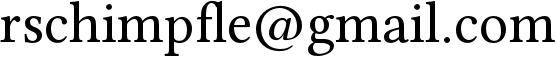
\includegraphics[height=2.2ex]{email-robert-schimpfle.png}

\vspace*{-0.35ex}

\smallskip

\noindent{}Diese Ausgabe wird durch die Comquent GmbH in Puchheim
gefördert, insbesondere durch Beratung und Unterstützung bei der
automatischen und kontinuierlichen Qualitätssicherung.

\clearpage

\subsection{Anmerkungen}

Verweise auf diese Ausgabe erhalten meist zusätzlich zur Seitenzahl
durch Doppelpunkte angehängte Zeilennummern. f.\ und ff.\ beziehen
sich in diesem Fall auf die Zeilennummer.

\theendnotes

\clearpage

\subsection{Literaturangaben}

\medskip

\bibentry{Beer-2016}{Ralf Beer}{Max Ludwig Mohr (1891–1937).
Biographische Rekonstruktion}{Martin-Luther-Universität Halle-Wittenberg,
Medizinischen Fakultät, Dissertation, Halle (Saale), 2016.\\
Verfügbar unter http://nbn-resolving.de/urn:nbn:de:gbv:3:4-17405\hspace*{\fill}\\
(Stand: \standonline{})}

\bibentry{Cronen-2017}{Thomas Cronen}{\buchautor{} (1891–1937). Rezeption
seines literarischen Werks}{Heidelberg 2017}

\bibentry{Humble-2011}{Jez Humble, David Farley}{Continuous Delivery}
{Boston 2011}

\bibentry{Mohr-1920}{\buchautor{}}{\buchtitel{}}{München 1920}

\bibentry{Mohr-1927}{\buchautor{}}{Venus in den Fischen}{Berlin 1927}

\bibentry{Mohr-1997}{\buchautor{}}{Das Einhorn, Romanfragment}{posthum hrsg.\ von Nicolas Humbert, Bonn 1997}

\bibentry{Pittner-1998}{Barbara Pittner}{\buchautor{} und die literarische Moderne}{Aachen 1998}

\bibentry{Reuss-2006}{Frederick Reuss}{Mohr: A Novel}{Denver 2006}

\bibentry{Steger-2013}{Florian Steger (Hg.)}{\buchautor{} (1891–1937) Korrespondenzen}{Heidelberg 2013}

\end{small}
